% KemdiCode MCP Server — IEEE Journal Paper v3.0.0 "Lorenz"
% Copyright (C) 2025-2026 Kemdi Sp. z o.o. (Dawid Irzyk)
% Licensed under GNU GPL v3

\documentclass[journal,10pt]{IEEEtran}

% ── Packages ──────────────────────────────────────────────────────
\usepackage[utf8]{inputenc}
\usepackage[T1]{fontenc}
\usepackage[english]{babel}
\usepackage{amsmath,amssymb}
\usepackage{graphicx}
\usepackage{tikz}
\usetikzlibrary{arrows.meta,positioning,fit,calc,shapes.geometric,decorations.pathreplacing,backgrounds,patterns}
\usepackage{booktabs}
\usepackage{tabularx}
\usepackage{multirow}
\usepackage{enumitem}
\usepackage{listings}
\usepackage{microtype}
\usepackage{cite}
\usepackage[ruled,linesnumbered,noend]{algorithm2e}
\usepackage{url}
\usepackage{hyperref}
\hypersetup{
  colorlinks=false,
  pdfborder={0 0 0},
  pdftitle={KemdiCode MCP v3: Lorenz-Inspired Context Compaction for AI-Assisted Software Engineering},
  pdfauthor={Dawid Irzyk},
}

% ── B&W color definitions ────────────────────────────────────────
\definecolor{darkgray}{gray}{0.25}
\definecolor{medgray}{gray}{0.55}
\definecolor{lightgray}{gray}{0.85}
\definecolor{verylightgray}{gray}{0.93}
\definecolor{codebg}{gray}{0.95}

% ── Listings ─────────────────────────────────────────────────────
\lstset{
  basicstyle=\ttfamily\scriptsize,
  backgroundcolor=\color{codebg},
  frame=single,
  rulecolor=\color{medgray},
  breaklines=true,
  tabsize=2,
  columns=fullflexible,
  xleftmargin=2mm,
  framexleftmargin=2mm,
  aboveskip=6pt,
  belowskip=4pt,
}

% ── Helpers ──────────────────────────────────────────────────────
\newcommand{\doi}[1]{\href{https://doi.org/#1}{\texttt{doi:#1}}}
\newcommand{\code}[1]{\texttt{#1}}
\newcommand{\layerthree}{L\textsubscript{3}}
\newcommand{\layertwo}{L\textsubscript{2}}
\newcommand{\layerone}{L\textsubscript{1}}

% ── Theorem-like environments ────────────────────────────────────
\newtheorem{definition}{Definition}
\newtheorem{property}{Property}
\newtheorem{invariant}{Invariant}

% ══════════════════════════════════════════════════════════════════
\begin{document}

\title{KemdiCode MCP v3: Lorenz-Inspired Context\\Compaction for AI-Assisted Software Engineering}

\author{Dawid~Irzyk,~M.Sc.~Eng.%
\thanks{D. Irzyk, M.Sc. Eng., is with Kemdi Sp. z o.o., Poland (e-mail: dawid@kemdi.pl).}%
\thanks{This work is licensed under the GNU General Public License v3.0. Source code is available at \url{https://git.kemdi.pl}.}}

\markboth{Kemdi Technical Report, 2026}%
{Irzyk: KemdiCode MCP v3: Lorenz-Inspired Context Compaction for AI-Assisted Software Engineering}

\maketitle

% ── Abstract ─────────────────────────────────────────────────────
\begin{abstract}
This paper presents KemdiCode MCP Server v3.0.0, an open-source Model Context Protocol~(MCP) server providing 107~specialized tools for AI cognition, multi-agent coordination, persistent memory, and distributed LLM orchestration. Version~3.0 introduces \emph{Lorenz-inspired context compaction}---three algorithms drawn from chaos theory and dynamical systems for intelligent context window management: Poincar\'{e} section phase detection using Jensen-Shannon divergence to identify topic transitions, Lorenz attractor orbit compression using TF-IDF cosine similarity to detect and collapse repeating reasoning patterns, and perturbation impact analysis measuring each item's contribution to the information landscape. Additionally, 39~tools duplicating native IDE AI capabilities (file operations, git, line editing, code review) have been removed, refocusing the server on capabilities that AI IDEs cannot provide natively. The three-layer distributed bus architecture (\layerthree~ClusterBus, \layertwo~DataFlowBus, \layerone~GlobalEventBus) and the eight-store cognition subsystem are retained and extended. Validation confirms 694~passing tests and compatibility with four major MCP clients.
\end{abstract}

\begin{IEEEkeywords}
Model Context Protocol, context compaction, Lorenz attractor, chaos theory, large language models, multi-agent systems, distributed systems, AI-assisted development
\end{IEEEkeywords}

% ══════════════════════════════════════════════════════════════════
\section{Introduction}
\label{sec:intro}

\IEEEPARstart{A}{I-assisted} development tools face a fundamental tension: as reasoning chains grow longer, the fixed context window forces lossy compression. Which thoughts to keep? Which to discard? This is the \emph{context compaction problem}---and it maps directly to sensitivity to initial conditions in chaotic dynamical systems.

In Lorenz's seminal meteorological model~\cite{lorenz1963}, infinitesimal perturbations to initial conditions produce exponentially divergent trajectories. Context compaction is the inverse problem: given a trajectory (thinking chain), find the minimal perturbation (compression) that preserves the system's qualitative behavior. If we remove the wrong thought, the AI's subsequent reasoning diverges catastrophically---the butterfly effect applied to cognition.

KemdiCode MCP Server v3.0.0 addresses this through three algorithms inspired by chaos theory and dynamical systems:

\begin{enumerate}[nosep,label=(\roman*)]
  \item \emph{Phase detection via Poincar\'{e} sections}: Identify topic transitions in thinking chains using Jensen-Shannon divergence~\cite{lin1991}. Phase boundaries carry maximum information and must be preserved during compaction.
  \item \emph{Orbit compression}: Detect repeating patterns in AI reasoning---analogous to orbits around the Lorenz attractor's ``eyes''---using TF-IDF cosine similarity matrices, and collapse duplicate cycles.
  \item \emph{Perturbation impact analysis}: Measure each item's contribution to the information landscape via JSD of the full context versus the context-without-item. Items with high perturbation impact are causal anchors.
\end{enumerate}

Concurrently, v3.0 removes 39~tools that duplicate capabilities provided natively by modern AI IDEs (Claude Code, Cursor, KiroCode, RooCode). File operations, git commands, line editing, code review, and project management tools have been excised, leaving 107~tools focused on cognition, multi-agent coordination, persistent memory, kanban task management, cluster bus with LLM magistrale, and structured output---capabilities that IDEs \emph{cannot} provide natively.

The remainder of this paper is organized as follows. Section~\ref{sec:related} surveys related work. Section~\ref{sec:lorenz} presents the Lorenz-inspired context compaction framework. Section~\ref{sec:arch} describes the system architecture. Section~\ref{sec:protocol} details the three protocol layers. Section~\ref{sec:magistrale} covers the LLM Magistrale. Section~\ref{sec:cognition} describes the cognition subsystem. Section~\ref{sec:tools} catalogs the tool categories. Section~\ref{sec:multiagent} addresses multi-agent coordination. Section~\ref{sec:security} discusses security. Section~\ref{sec:eval} presents the evaluation. Section~\ref{sec:conclusion} concludes.

% ══════════════════════════════════════════════════════════════════
\section{Related Work}
\label{sec:related}

The Model Context Protocol builds on the architectural patterns established by the Language Server Protocol~(LSP)~\cite{lsp2016}, which standardized language intelligence features across IDEs. While LSP focuses on language-specific operations (completion, diagnostics, refactoring), MCP generalizes the client-server pattern to arbitrary tool invocations for AI assistants.

Multi-agent LLM frameworks have been explored extensively. AutoGen~\cite{wu2023autogen} enables multi-agent conversation through a conversable agent abstraction. MetaGPT~\cite{hong2023metagpt} introduces role-based agent coordination. Li~et~al.~\cite{li2024multiagent} survey workflow patterns and infrastructure requirements. Guo~et~al.~\cite{guo2024ijcai} provide a comprehensive taxonomy of multi-agent architectures. KemdiCode differs from these frameworks by operating at the protocol level---it exposes coordination primitives as MCP tools rather than implementing a fixed agent architecture.

Context window management has received increasing attention as LLMs tackle multi-step reasoning tasks. Recursive summarization~\cite{wu2021recursively} compresses conversation history but loses structural information. Retrieval-augmented generation~\cite{lewis2020rag} sidesteps the problem by keeping a vector store, but cannot preserve causal reasoning chains. Our approach treats the thinking chain as a dynamical trajectory and applies tools from chaos theory to identify which elements are structurally essential.

For distributed messaging, Redis Pub/Sub~\cite{redis} provides the foundation for KemdiCode's inter-cluster communication. Tree-sitter~\cite{treesitter} provides the AST infrastructure. Secret sharing follows Shamir's original construction~\cite{shamir1979}.

% ══════════════════════════════════════════════════════════════════
\section{Lorenz-Inspired Context Compaction}
\label{sec:lorenz}

The central insight of v3.0 is that \emph{context compaction is a sensitivity-to-initial-conditions problem}. The Lorenz system~\cite{lorenz1963}:

\begin{equation}
\dot{x} = \sigma(y - x), \quad \dot{y} = x(\rho - z) - y, \quad \dot{z} = xy - \beta z
\label{eq:lorenz}
\end{equation}

\noindent exhibits three properties that map directly to the context compaction problem:

\begin{enumerate}[nosep]
\item \textbf{Sensitivity to initial conditions}: Removing a critical thought (perturbing the initial state) causes the AI's subsequent reasoning to diverge exponentially.
\item \textbf{Strange attractor structure}: AI reasoning tends to orbit around a finite set of conceptual ``eyes'' (key ideas), tracing similar but not identical paths---creating compressible redundancy.
\item \textbf{Phase transitions}: The Lorenz system exhibits rapid transitions between the two attractor lobes, analogous to topic switches in thinking chains.
\end{enumerate}

We formalize three algorithms that exploit these properties.

\subsection{Phase Detection via Poincar\'{e} Sections}
\label{sec:phase}

In dynamical systems, a Poincar\'{e} section is a hyperplane transverse to the flow, used to reduce continuous dynamics to a discrete map~\cite{poincare1890}. We apply this concept to thinking chains: the ``flow'' is the sequence of thoughts, and ``Poincar\'{e} sections'' are the points where the topic changes direction.

\begin{definition}[Phase Boundary]
\label{def:phase}
Given a thinking chain $\mathcal{T} = (t_1, t_2, \ldots, t_n)$ where each $t_i$ has content $c_i$, a \emph{phase boundary} exists between $t_i$ and $t_{i+1}$ if:
\begin{equation}
\text{JSD}\bigl(P(c_i) \| P(c_{i+1})\bigr) > \tau_{\text{phase}}
\label{eq:phase}
\end{equation}
where $P(c)$ is the token probability distribution of content $c$ and $\tau_{\text{phase}} = 0.35$ is the phase detection threshold.
\end{definition}

The Jensen-Shannon divergence~\cite{lin1991} is defined as:

\begin{equation}
\text{JSD}(P \| Q) = \frac{1}{2} D_{\text{KL}}(P \| M) + \frac{1}{2} D_{\text{KL}}(Q \| M)
\label{eq:jsd}
\end{equation}

\noindent where $M = \frac{1}{2}(P + Q)$ is the mixture distribution and $D_{\text{KL}}$ is the Kullback-Leibler divergence:

\begin{equation}
D_{\text{KL}}(P \| Q) = \sum_{x} P(x) \ln \frac{P(x)}{Q(x)}
\label{eq:kl}
\end{equation}

The token probability distribution $P(c)$ is computed by tokenizing the content (lowercased, stop-words removed, minimum 2~characters), computing term frequencies, and normalizing to a probability distribution.

\subsubsection{Preservation Strategy}

Phase detection identifies which thoughts to \emph{preserve} during compaction:

\begin{itemize}[nosep]
\item The first and last thoughts (trajectory endpoints).
\item All phase boundary thoughts (maximum information content at topic transitions).
\item The highest-confidence thought within each phase segment (representative of the segment's conclusion).
\end{itemize}

\begin{property}[Phase Boundary Information Maximum]
\label{prop:boundary}
At a phase boundary $b_k$, the mutual information between the content and the ``topic'' variable is locally maximal:
\begin{equation}
I(c_{b_k}; \text{topic}) \geq I(c_j; \text{topic}) \quad \forall j \in [b_{k-1}+1, b_{k+1}-1]
\label{eq:mutual}
\end{equation}
This follows from the JSD threshold: high JSD indicates that the token distributions before and after the boundary are maximally different, meaning the boundary thought carries the most information about the transition.
\end{property}

The mutual information is approximated using:

\begin{equation}
I(X; Y) \approx H(X) + H(Y) - H(X, Y)
\label{eq:mi}
\end{equation}

\noindent where $H$ is the Shannon entropy~\cite{shannon1948}:

\begin{equation}
H(P) = -\sum_{x} P(x) \log_2 P(x)
\label{eq:entropy}
\end{equation}

\subsection{Orbit Compression}
\label{sec:orbit}

In the Lorenz system, trajectories orbit around two ``eyes'' of the strange attractor, tracing similar but not identical paths. Each orbit is qualitatively similar to the previous one. Applied to AI reasoning, an \emph{orbit} is a repeating pattern where the model revisits the same conceptual territory from slightly different angles.

\begin{definition}[Orbital Cycle]
\label{def:orbit}
A subsequence $(t_{s}, t_{s+1}, \ldots, t_{s+L-1})$ of length $L$ is an \emph{orbital cycle} if there exists a subsequent subsequence $(t_{s+L}, \ldots, t_{s+2L-1})$ such that:
\begin{equation}
\frac{1}{L} \sum_{k=0}^{L-1} \text{sim}(t_{s+k}, t_{s+L+k}) \geq \tau_{\text{orbit}}
\label{eq:orbit}
\end{equation}
where $\text{sim}(t_i, t_j)$ is the TF-IDF cosine similarity between thoughts $t_i$ and $t_j$, and $\tau_{\text{orbit}} = 0.5$ is the similarity threshold.
\end{definition}

\subsubsection{Detection Algorithm}

The orbit detection algorithm operates in three phases:

\begin{enumerate}[nosep]
\item \textbf{Similarity matrix construction}: Compute the $n \times n$ pairwise TF-IDF cosine similarity matrix $\mathbf{S}$ where $S_{ij} = \text{sim}(t_i, t_j)$.
\item \textbf{Greedy cycle search}: For cycle lengths $L \in [L_{\max}, L_{\min}]$ (longer first), scan starting positions and check for repetitions using (\ref{eq:orbit}). Mark claimed indices to prevent overlap.
\item \textbf{Compression}: For each detected cycle with $r$ repetitions, keep the first occurrence and prune the remaining $r-1$ copies.
\end{enumerate}

The TF-IDF cosine similarity is computed as:

\begin{equation}
\text{sim}(t_i, t_j) = \frac{\mathbf{v}_i \cdot \mathbf{v}_j}{|\mathbf{v}_i| \cdot |\mathbf{v}_j|}
\label{eq:cosine}
\end{equation}

\noindent where $\mathbf{v}_i$ is the TF-IDF vector of thought $t_i$, with term frequency $\text{TF}(w, t) = \text{count}(w, t) / |t|$ and inverse document frequency $\text{IDF}(w) = \log(N / \text{df}(w))$, where $N$ is the total number of thoughts and $\text{df}(w)$ is the number of thoughts containing word $w$.

Algorithm~\ref{alg:orbit} formalizes the procedure.

\begin{algorithm}[!t]
\caption{Orbit Compression}\label{alg:orbit}
\SetAlgoLined
\SetKwInOut{Input}{Input}
\SetKwInOut{Output}{Output}
\Input{thoughts $\mathcal{T} = (t_1, \ldots, t_n)$, threshold $\tau$}
\Output{keep indices $\mathcal{K}$, prune indices $\mathcal{P}$}
$\mathbf{S} \leftarrow \text{computeSimilarityMatrix}(\mathcal{T})$\;
$\text{claimed} \leftarrow \emptyset$\;
$\text{orbits} \leftarrow []$\;
\For{$L \leftarrow \min(L_{\max}, \lfloor n/2 \rfloor)$ \KwTo $L_{\min}$}{
  \For{$s \leftarrow 0$ \KwTo $n - L \cdot R_{\min}$}{
    \If{$\exists k \in [s, s+L): k \in \text{claimed}$}{\textbf{continue}}
    $(r, \bar{S}) \leftarrow \text{detectRepetitions}(\mathbf{S}, s, L, \tau)$\;
    \If{$r \geq R_{\min}$}{
      $\text{claimed} \leftarrow \text{claimed} \cup \{s, \ldots, s + r \cdot L - 1\}$\;
      $\text{orbits.push}(s, L, r, \bar{S})$\;
    }
  }
}
$\mathcal{P} \leftarrow \bigcup_{\text{orbit}} \text{orbit.pruneIndices}$\;
$\mathcal{K} \leftarrow \{1, \ldots, n\} \setminus \mathcal{P}$\;
\end{algorithm}

\noindent with constants $L_{\min} = 2$, $L_{\max} = 10$, $R_{\min} = 2$.

\subsection{Perturbation Impact Analysis}
\label{sec:perturbation}

The perturbation impact of an item $t_k$ measures how much its removal changes the information landscape of the remaining context:

\begin{definition}[Perturbation Impact]
\label{def:perturbation}
For a context set $\mathcal{C} = \{t_1, \ldots, t_n\}$, the perturbation impact of item $t_k$ is:
\begin{equation}
\Pi(t_k) = \text{JSD}\bigl(P(\mathcal{C}) \| P(\mathcal{C} \setminus \{t_k\})\bigr)
\label{eq:perturbation}
\end{equation}
where $P(\mathcal{C})$ is the aggregate token distribution of all items in $\mathcal{C}$.
\end{definition}

Items are ranked by $\Pi(t_k)$ in descending order. High-impact items are \emph{causal anchors}---their removal would maximally perturb the system's trajectory, analogous to the critical initial conditions in the Lorenz system.

\begin{property}[Perturbation--Entropy Relationship]
\label{prop:perturbation}
For a uniform context (all items have identical content), $\Pi(t_k) = 0$ for all $k$. For a maximally diverse context (each item introduces unique vocabulary), $\Pi(t_k)$ correlates with the information density:
\begin{equation}
\rho(t_k) = \frac{H(P(t_k))}{\log_2 |V(t_k)|}
\label{eq:density}
\end{equation}
where $|V(t_k)|$ is the vocabulary size of item $t_k$. Items with $\rho \approx 1$ have near-uniform token distributions and contribute maximally to the context's information landscape.
\end{property}

\subsection{Integrated Compaction Pipeline}

The three algorithms are composed into a compaction pipeline:

\begin{enumerate}[nosep]
\item \textbf{Phase detection}: Identify phase boundaries and mark boundary thoughts as \emph{protected}.
\item \textbf{Orbit compression}: Within each phase segment, detect and collapse orbital cycles.
\item \textbf{Perturbation ranking}: Rank remaining unprotected thoughts by perturbation impact. Evict thoughts with lowest $\Pi$ until the context budget is met.
\end{enumerate}

The composition ensures that:
\begin{itemize}[nosep]
\item Phase boundaries (maximum-information transitions) are never evicted.
\item Redundant orbits are collapsed before perturbation ranking, preventing duplicate content from inflating impact scores.
\item The final eviction uses information-theoretic ranking, not heuristic recency/frequency.
\end{itemize}

\subsection{Additional CTC-Inspired Algorithms}
\label{sec:ctc}

The cognition module includes additional algorithms inspired by Closed Timelike Curves~(CTC) from general relativity:

\begin{description}[nosep,style=unboxed,leftmargin=0pt,font=\normalfont\itshape]
\item[Causal DAG analysis.] Constructs a directed acyclic graph of dependencies between cognition items and computes the causal core---the minimal set of items needed to reconstruct all others---using transitive reduction.

\item[Fixed-point detection.] Iteratively compacts a thinking chain until convergence, defined as:
\begin{equation}
|C_{i+1}| \geq |C_i| \cdot (1 - \epsilon), \quad \epsilon = 0.05
\label{eq:fixedpoint}
\end{equation}
This mirrors the Novikov self-consistency principle: the compacted result must be a fixed point that regenerates itself under further compaction.

\item[Gravitational TTL.] Assigns time-to-live based on item ``mass'' (information density $\times$ link count), analogous to gravitational time dilation:
\begin{equation}
\text{TTL}(t_k) = \text{TTL}_{\text{base}} \cdot \left(1 + \alpha \cdot m(t_k)\right)
\label{eq:gttl}
\end{equation}
where $m(t_k)$ is the normalized mass and $\alpha = 0.5$ is the amplification factor. High-mass items live longer.
\end{description}

% ══════════════════════════════════════════════════════════════════
\section{System Architecture}
\label{sec:arch}

Fig.~\ref{fig:arch} shows the high-level system architecture. The server is organized into five principal layers: transport, session management, tool registry, bus architecture, and shared infrastructure.

\begin{figure}[!t]
\centering
\resizebox{\columnwidth}{!}{%
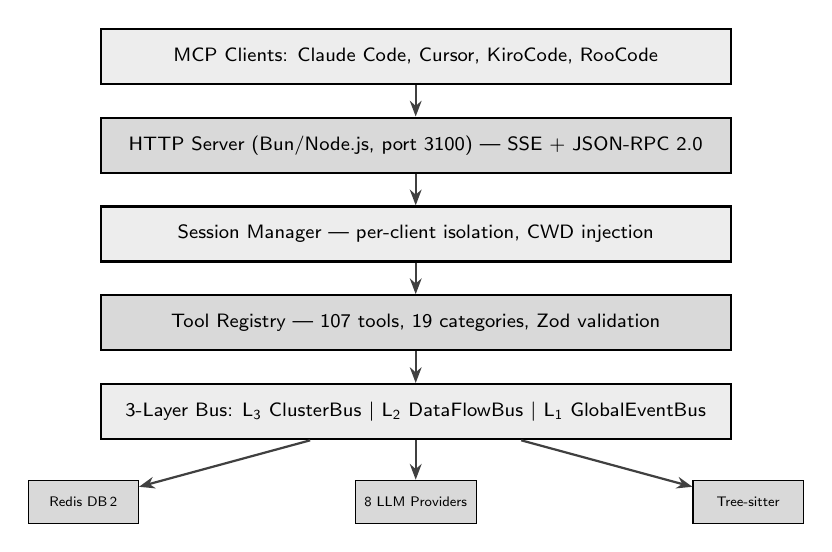
\begin{tikzpicture}[
  node distance=0.4cm,
  box/.style={draw, thick, minimum width=80mm, minimum height=7mm, font=\sffamily\scriptsize, align=center, fill=#1},
  smallbox/.style={draw, minimum width=14mm, minimum height=5.5mm, font=\sffamily\tiny, align=center, fill=#1},
  arr/.style={-{Stealth[length=2mm]}, thick, color=darkgray},
]
  \node[box=verylightgray] (clients) {MCP Clients: Claude Code, Cursor, KiroCode, RooCode};
  \node[box=lightgray, below=of clients] (http) {HTTP Server (Bun/Node.js, port 3100) --- SSE + JSON-RPC 2.0};
  \node[box=verylightgray, below=of http] (session) {Session Manager --- per-client isolation, CWD injection};
  \node[box=lightgray, below=of session] (registry) {Tool Registry --- 107 tools, 19 categories, Zod validation};
  \node[box=verylightgray, below=of registry] (bus) {3-Layer Bus: \layerthree{} ClusterBus $\mid$ \layertwo{} DataFlowBus $\mid$ \layerone{} GlobalEventBus};
  \node[smallbox=lightgray, below left=0.5cm and -0.5cm of bus] (redis) {Redis DB\,2};
  \node[smallbox=lightgray, below=0.5cm of bus] (llm) {8 LLM Providers};
  \node[smallbox=lightgray, below right=0.5cm and -0.5cm of bus] (ts) {Tree-sitter};

  \draw[arr] (clients) -- (http);
  \draw[arr] (http) -- (session);
  \draw[arr] (session) -- (registry);
  \draw[arr] (registry) -- (bus);
  \draw[arr] (bus) -- (redis);
  \draw[arr] (bus) -- (llm);
  \draw[arr] (bus) -- (ts);
\end{tikzpicture}}%
\caption{High-level system architecture. Version~3.0 reduces the tool registry from 147 to 107 tools by removing capabilities provided natively by IDE AI clients.}
\label{fig:arch}
\end{figure}

\subsection{Transport Layer}

The server implements the MCP Streamable~HTTP transport, exposing the endpoints listed in Table~\ref{tab:endpoints}. Communication follows JSON-RPC~2.0 with the MCP method extensions. Server-Sent Events~(SSE)~\cite{sse2015} provide the server-to-client notification channel.

\begin{table}[!t]
\centering
\caption{HTTP Endpoints}
\label{tab:endpoints}
\begin{tabular}{@{}llp{32mm}@{}}
\toprule
\textbf{Method} & \textbf{Path} & \textbf{Purpose} \\
\midrule
\texttt{GET}  & \texttt{/sse}        & SSE notification stream \\
\texttt{POST} & \texttt{/message}    & JSON-RPC tool invocations \\
\texttt{GET}  & \texttt{/stream/:id} & Per-request execution stream \\
\texttt{GET}  & \texttt{/health}     & Health check and uptime \\
\texttt{GET}  & \texttt{/tools}      & Tool listing with schemas \\
\texttt{GET}  & \texttt{/mcp}        & Streamable HTTP endpoint \\
\bottomrule
\end{tabular}
\end{table}

\subsection{Tool Registry}

The tool registry manages 107~tools through a unified \code{UnifiedTool} interface. Each tool defines its input schema using Zod~\cite{zod}, which is converted to JSON~Schema for the MCP protocol. Lazy loading ensures that tool implementations are instantiated on first invocation. The availability checker reports tool health with soft and force modes, suggesting fallback alternatives when dependencies are unavailable.

\subsection{Tool Removal Rationale (v3.0)}
\label{sec:removal}

Version~3.0 removes 39~tools across 8~categories: file operations~(9), git~(9), line editing~(4), symbol editing~(3), code navigation~(2), code modification~(5), AI specialized~(2), and project management~(5). These tools duplicated capabilities that modern AI IDEs provide natively:

\begin{itemize}[nosep]
\item \textbf{Claude Code}: built-in \code{Read}, \code{Write}, \code{Edit}, \code{Bash}, \code{Glob}, \code{Grep} tools.
\item \textbf{Cursor}: native file editing, terminal, and code navigation.
\item \textbf{KiroCode/RooCode}: equivalent built-in tool sets.
\end{itemize}

The internal utility modules (\code{utils/file-utils.ts}, \code{utils/git-utils.ts}) are preserved, as they are used by remaining tools (e.g., \code{write-tests} uses file reading, \code{smart-handoff} uses git status).

% ══════════════════════════════════════════════════════════════════
\section{Protocol Layer Architecture}
\label{sec:protocol}

The communication infrastructure consists of three layers connected by anti-amplification bridges. Fig.~\ref{fig:bus} illustrates the layered design.

\begin{figure}[!t]
\centering
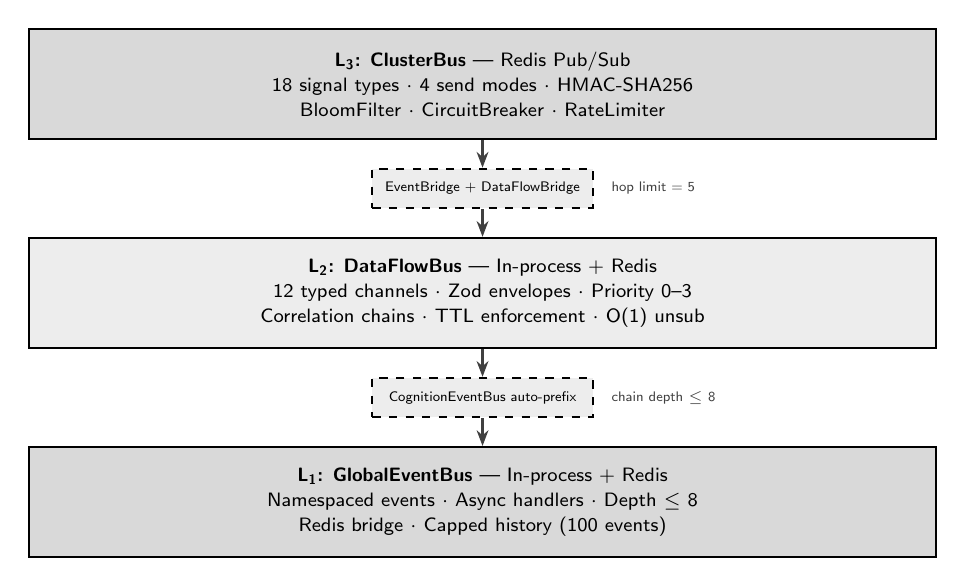
\begin{tikzpicture}[
  node distance=0.35cm,
  layer/.style={draw, thick, minimum width=\columnwidth-6mm, font=\sffamily\scriptsize, align=center, minimum height=14mm},
  bridge/.style={draw, dashed, thick, minimum width=28mm, minimum height=5mm, font=\sffamily\tiny, fill=verylightgray},
  arr/.style={-{Stealth[length=2mm]}, thick, color=darkgray},
]
  % L3
  \node[layer, fill=lightgray] (l3) {
    \textbf{\layerthree: ClusterBus} --- Redis Pub/Sub\\[1pt]
    18 signal types $\cdot$ 4 send modes $\cdot$ HMAC-SHA256\\[1pt]
    BloomFilter $\cdot$ CircuitBreaker $\cdot$ RateLimiter
  };

  \node[bridge, below=of l3] (b32) {EventBridge + DataFlowBridge};

  \node[layer, fill=verylightgray, below=of b32] (l2) {
    \textbf{\layertwo: DataFlowBus} --- In-process + Redis\\[1pt]
    12 typed channels $\cdot$ Zod envelopes $\cdot$ Priority 0--3\\[1pt]
    Correlation chains $\cdot$ TTL enforcement $\cdot$ O(1) unsub
  };

  \node[bridge, below=of l2] (b21) {CognitionEventBus auto-prefix};

  \node[layer, fill=lightgray, below=of b21] (l1) {
    \textbf{\layerone: GlobalEventBus} --- In-process + Redis\\[1pt]
    Namespaced events $\cdot$ Async handlers $\cdot$ Depth $\leq$ 8\\[1pt]
    Redis bridge $\cdot$ Capped history (100 events)
  };

  \draw[arr] (l3.south) -- (b32.north);
  \draw[arr] (b32.south) -- (l2.north);
  \draw[arr] (l2.south) -- (b21.north);
  \draw[arr] (b21.south) -- (l1.north);

  \node[font=\sffamily\tiny, right=1mm of b32, text=darkgray] {hop limit = 5};
  \node[font=\sffamily\tiny, right=1mm of b21, text=darkgray] {chain depth $\leq$ 8};
\end{tikzpicture}
\caption{Three-layer bus architecture with anti-amplification bridges.}
\label{fig:bus}
\end{figure}

\subsection{\layerthree: ClusterBus}
\label{sec:l3}

The ClusterBus enables inter-cluster communication over Redis Pub/Sub~\cite{redis} with 18~signal types organized into four namespaces plus CI/CD. Four send modes are supported: unicast, broadcast, routed (via MetaRouter with tag-based boolean logic), and multicast (fan-out to multiple targets).

\subsubsection{Dual-Layer Deduplication}

A bounded set of 2{,}000 recent signal IDs provides exact deduplication. Overflow is handled by a bloom filter~\cite{bloom1970} configured for 20{,}000~items at 0.1\% false-positive rate:

\begin{equation}
m = -\frac{n \ln p}{(\ln 2)^2}, \quad k = \frac{m}{n} \ln 2
\label{eq:bloom}
\end{equation}

\subsubsection{HMAC Authentication}

Signals are authenticated using HMAC-SHA256 with constant-time comparison to prevent timing side-channel attacks.

\subsubsection{SignalFlowController}

Governs throughput through rate limiting, circuit breaking~\cite{nygard2007} (closed $\to$ open $\to$ half-open automaton), priority filtering, and backpressure control.

\subsection{\layertwo: DataFlowBus}
\label{sec:l2}

12~typed channels with Zod-validated envelopes, correlation tracking, priority 0--3, and TTL enforcement. Messages are persisted to Redis under \code{mcp:dataflow:\{channel\}}.

\subsection{\layerone: GlobalEventBus}
\label{sec:l1}

In-process event emitter with namespaced events (\code{module:category:action}), async dispatch with chain depth limit of~8, and Redis bridge for cross-session propagation.

\subsection{Anti-Amplification Bridges}
\label{sec:bridges}

Four guards prevent feedback loops: hop counter (max~5), source prefix filtering, per-bridge dedup set, and chain depth limiting.

\begin{invariant}[Signal Termination]
\label{inv:termination}
For any signal $s$, the total copies across all layers is bounded by:
\begin{equation}
|C(s)| \leq H_{\max} \cdot D_{\max} = 5 \times 8 = 40
\label{eq:termination}
\end{equation}
In practice, deduplication reduces this to $|C(s)| \leq 3$.
\end{invariant}

% ══════════════════════════════════════════════════════════════════
\section{LLM Magistrale}
\label{sec:magistrale}

The LLM Magistrale orchestrates distributed prompt execution across multiple clusters. Fig.~\ref{fig:magistrale} illustrates the dispatch flow.

\begin{figure}[!t]
\centering
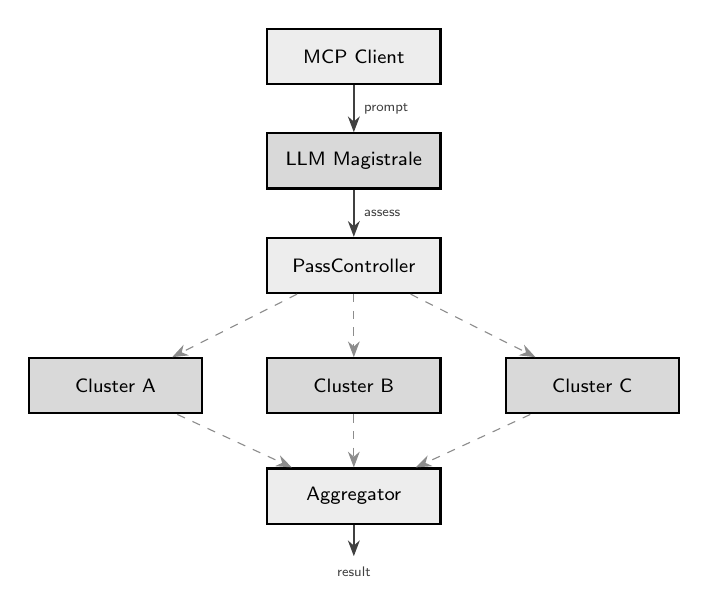
\begin{tikzpicture}[
  node distance=0.6cm,
  box/.style={draw, thick, minimum width=22mm, minimum height=7mm, font=\sffamily\scriptsize, align=center, fill=#1},
  arr/.style={-{Stealth[length=2mm]}, thick, color=darkgray},
  darr/.style={-{Stealth[length=2mm]}, dashed, color=medgray},
]
  \node[box=verylightgray] (client) {MCP Client};
  \node[box=lightgray, below=of client] (mag) {LLM Magistrale};
  \node[box=verylightgray, below=of mag] (pass) {PassController};

  \node[box=lightgray, below left=0.8cm and 0.8cm of pass] (ca) {Cluster A};
  \node[box=lightgray, below=0.8cm of pass] (cb) {Cluster B};
  \node[box=lightgray, below right=0.8cm and 0.8cm of pass] (cc) {Cluster C};

  \node[box=verylightgray, below=2.2cm of pass] (agg) {Aggregator};

  \draw[arr] (client) -- node[right, font=\sffamily\tiny] {prompt} (mag);
  \draw[arr] (mag) -- node[right, font=\sffamily\tiny] {assess} (pass);
  \draw[darr] (pass) -- (ca);
  \draw[darr] (pass) -- (cb);
  \draw[darr] (pass) -- (cc);
  \draw[darr] (ca) -- (agg);
  \draw[darr] (cb) -- (agg);
  \draw[darr] (cc) -- (agg);
  \draw[arr] (agg.south) -- ++(0,-0.4) node[below, font=\sffamily\tiny] {result};
\end{tikzpicture}
\caption{LLM Magistrale dispatch flow. Solid arrows: control flow; dashed: async ClusterBus signals.}
\label{fig:magistrale}
\end{figure}

\subsection{Aggregation Strategies}

Four strategies are supported: \emph{first-wins} (latency-optimized), \emph{best-of-$n$} with composite scoring, \emph{consensus} (weighted Jaccard similarity, threshold 0.6), and \emph{fallback-chain} (sequential priority). The composite score is:

\begin{equation}
S = w_q \cdot Q + w_d \cdot D + w_t \cdot T - w_l \cdot L
\label{eq:score}
\end{equation}

\noindent with default weights $w_q = 0.45$, $w_d = 0.25$, $w_t = 0.15$, $w_l = 0.15$.

\subsection{PassController}

Three strategies govern multi-pass execution: \emph{min-passes} (LLM self-assesses), \emph{quality-target} (iterate until $Q_i \geq Q_{\text{target}}$), and \emph{fixed} (exact $N$ passes). Budget capping limits \code{minPasses} to \code{maxPasses}.

% ══════════════════════════════════════════════════════════════════
\section{Cognition Subsystem}
\label{sec:cognition}

The cognition layer provides persistent AI self-awareness through eight primary stores, two auxiliary analyzers, and a cross-linking mechanism. Fig.~\ref{fig:cognition} shows the store interconnections.

\begin{figure}[!t]
\centering
\resizebox{\columnwidth}{!}{%
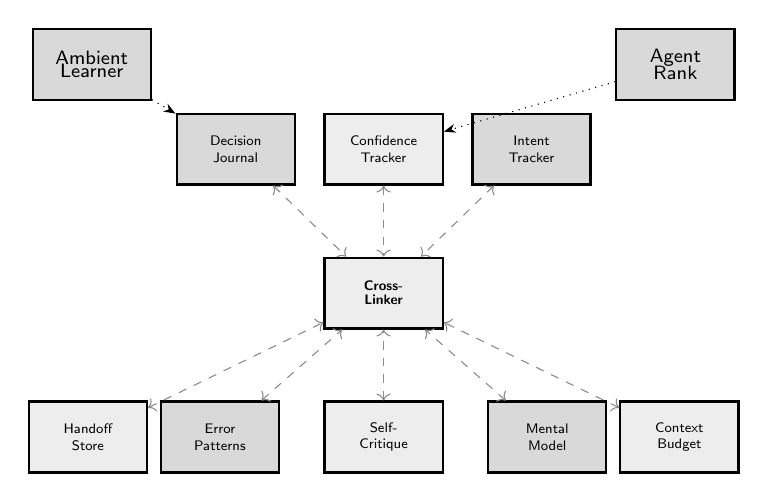
\begin{tikzpicture}[
  node distance=0.45cm and 0.35cm,
  store/.style={draw, thick, minimum width=15mm, minimum height=9mm, font=\sffamily\tiny, align=center, fill=#1},
  link/.style={<->, thin, dashed, color=medgray},
]
  \node[store=lightgray]      (dec)    {Decision\\Journal};
  \node[store=verylightgray, right=of dec]  (conf)   {Confidence\\Tracker};
  \node[store=lightgray, right=of conf] (intent) {Intent\\Tracker};

  \node[store=verylightgray, below=0.9cm of conf] (xlink) {\textbf{Cross-}\\[-1pt]\textbf{Linker}};

  \node[store=lightgray, below left=0.9cm and 0.55cm of xlink]   (err)   {Error\\Patterns};
  \node[store=verylightgray, below=0.9cm of xlink]               (crit)  {Self-\\Critique};
  \node[store=lightgray, below right=0.9cm and 0.55cm of xlink]  (model) {Mental\\Model};

  \node[store=verylightgray, left=0.15cm of err] (hand) {Handoff\\Store};
  \node[store=verylightgray, right=0.15cm of model] (budget) {Context\\Budget};

  \node[store=lightgray, above left=0.15cm and 0.3cm of dec] (ambient) {\scriptsize Ambient\\[-1pt]\scriptsize Learner};
  \node[store=lightgray, above right=0.15cm and 0.3cm of intent] (rank) {\scriptsize Agent\\[-1pt]\scriptsize Rank};

  \draw[link] (dec) -- (xlink);
  \draw[link] (conf) -- (xlink);
  \draw[link] (intent) -- (xlink);
  \draw[link] (err) -- (xlink);
  \draw[link] (crit) -- (xlink);
  \draw[link] (model) -- (xlink);
  \draw[link] (hand) -- (xlink);
  \draw[link] (budget) -- (xlink);

  \draw[-{Stealth[length=1.5mm]}, thin, dotted] (ambient) -- (dec);
  \draw[-{Stealth[length=1.5mm]}, thin, dotted] (rank) -- (conf);
\end{tikzpicture}}%
\caption{Cognition stores interconnected via CognitionCrossLinker.}
\label{fig:cognition}
\end{figure}

The eight primary stores are: DecisionJournal (structured decisions with outcome tracking), ConfidenceTracker (calibrated scores with ECE monitoring), IntentTracker (hierarchical goals with TF-IDF drift detection), ErrorPatternDB (cross-session error database), SelfCritiqueStore (post-task reflections), MentalModelStore (component-relationship architecture maps), HandoffStore (auto-enriched session snapshots), and ContextBudgetManager (token estimation with relevance scoring).

Agent ranking uses a composite score with five tiers (bronze through diamond):

\begin{equation}
\text{Score} = 0.4 \cdot S_r + 0.3 \cdot C_t + 0.2 \cdot A_s + 0.1 \cdot C_o
\label{eq:rank}
\end{equation}

\noindent with exponential temporal decay $\text{Score}(t) = \text{Score}_0 \cdot 0.95^{\Delta t / \tau}$.

Nine reactive event handlers create feedback loops between stores (e.g., \code{decision:recorded} auto-creates confidence records, \code{intent:drifted} triggers self-critique).

% ══════════════════════════════════════════════════════════════════
\section{Tool Categories}
\label{sec:tools}

Table~\ref{tab:tools} enumerates all 19~tool categories with counts and representative tools.

\begin{table}[!t]
\centering
\caption{Tool Categories (107 Total)}
\label{tab:tools}
\renewcommand{\arraystretch}{0.95}
\begin{tabular}{@{}lcp{28mm}@{}}
\toprule
\textbf{Category} & \textbf{\#} & \textbf{Key Tools} \\
\midrule
Core AI           & 6  & \code{ask-ai}, \code{plan}, \code{build} \\
Code Intelligence & 4  & \code{find-definition}, \code{semantic-search} \\
Multi-LLM         & 3  & \code{multi-prompt}, \code{consensus} \\
Cognition         & 8  & \code{decision-journal}, \code{confidence} \\
Multi-Agent       & 10 & \code{agent-init}, \code{agent-rank} \\
Context           & 3  & \code{shared-thoughts}, \code{feedback} \\
Kanban Tasks      & 13 & \code{task-create}, \code{task-cluster} \\
Kanban Workspaces & 5  & \code{workspace-create}, \code{-join} \\
Kanban Boards     & 7  & \code{board-create}, \code{board-workflow} \\
Project Memory    & 8  & \code{write-memory}, \code{checkpoint-save} \\
Recursive         & 4  & \code{invoke-tool}, \code{orchestrate} \\
Session           & 6  & \code{session-recover}, \code{session-create} \\
Thinking          & 1  & \code{thinking-chain} \\
Knowledge Graph   & 4  & \code{graph-query}, \code{loci-recall} \\
Cluster Bus       & 8  & \code{bus-status}, \code{-magistrale} \\
MPC Security      & 4  & \code{mpc-split}, \code{mpc-reconstruct} \\
RL Learning       & 2  & \code{rl-reward-stats} \\
MCP Client        & 3  & \code{client-sampling}, \code{client-elicit} \\
System            & 8  & \code{env-info}, \code{tool-health}, \code{ping} \\
\bottomrule
\end{tabular}
\end{table}

% ══════════════════════════════════════════════════════════════════
\section{Multi-Agent Coordination}
\label{sec:multiagent}

KemdiCode supports multi-agent workflows through four mechanisms:

\begin{description}[nosep,style=unboxed,leftmargin=0pt,font=\normalfont\itshape]
\item[Agent Registry.] Agents register with role, capabilities, and status. Discovery via \code{agent-list}; monitoring via \code{monitor} with five views (overview, agents, tasks, hierarchy, activity).

\item[Message Passing.] \code{agent-inject} sends context to specific agents via Redis Pub/Sub. \code{agent-alert} broadcasts to all agents. \code{shared-thoughts} provides a collective knowledge base.

\item[Kanban System.] Hierarchical task management: workspaces contain boards, boards contain tasks with subtask support. Role-based membership (owner, admin, member, viewer) controls access.

\item[Task Intelligence.] \code{task-cluster} uses LLM-driven semantic clustering. \code{task-complexity} provides AI-powered difficulty estimation.
\end{description}

% ══════════════════════════════════════════════════════════════════
\section{Security}
\label{sec:security}

Security mechanisms include: Zod schema validation on all inputs, path traversal protection via \code{validatePathSafe()}, Redis JSON parsing with prototype pollution protection, HMAC-SHA256 cluster signal authentication with constant-time comparison, Shamir's Secret Sharing~\cite{shamir1979} for distributed secret management, and ReDoS prevention through regex pattern length caps.

% ══════════════════════════════════════════════════════════════════
\section{LLM Provider Integration}
\label{sec:providers}

Eight providers with unified \code{provider:model:thinking} syntax: Anthropic~(\code{a}), OpenAI~(\code{o}), Gemini~(\code{g}) with native SDKs, and Groq~(\code{q}), DeepSeek~(\code{d}), Ollama~(\code{l}), OpenRouter~(\code{r}), Perplexity~(\code{p}) via OpenAI-compatible adapters. Three-tier routing (primary/research/fallback), lazy initialization, hot-reload, and structured output via \code{generateObject()} with Zod schemas and \code{jsonrepair}.

% ══════════════════════════════════════════════════════════════════
\section{Evaluation}
\label{sec:eval}

\subsection{Test Suite}

694~passing tests across 29~test files covering all tool categories, bus layers, cognition stores, context compaction algorithms, and edge cases. Tests are executed via Vitest~\cite{vitest} with the V8 coverage provider.

\subsection{Client Compatibility}

Verified with four MCP clients: Claude Code (primary), Cursor, KiroCode, and RooCode.

\subsection{Infrastructure}

Dual-runtime support (Bun and Node.js). Tree-sitter~\cite{treesitter} WASM parsers for 19~languages. All persistent state uses Redis DB~2 with 10~key namespaces.

\subsection{Tool Reduction Impact}

The removal of 39~tools reduces the server's surface area by 27\%. The remaining 107~tools have zero overlap with native IDE capabilities. Startup time improves proportionally due to fewer lazy-loadable modules. No functional regression: all removed capabilities are available natively in supported MCP clients.

% ══════════════════════════════════════════════════════════════════
\section{Conclusion}
\label{sec:conclusion}

KemdiCode MCP Server v3.0.0 demonstrates two key contributions. First, that chaos theory and dynamical systems provide a rigorous framework for AI context compaction: Poincar\'{e} section phase detection identifies information-dense topic transitions, Lorenz attractor orbit compression eliminates redundant reasoning cycles, and perturbation impact analysis quantifies each thought's structural importance. Together, these algorithms replace heuristic recency-based eviction with information-theoretic compression.

Second, that MCP tool servers should focus on capabilities that AI IDEs cannot provide natively. By removing 39~redundant tools, v3.0 achieves a 27\% reduction in tool count while improving focus: the remaining 107~tools cover cognition, multi-agent coordination, persistent memory, distributed LLM orchestration, and context compaction---domains where protocol-level tooling is essential.

The three-layer bus architecture, eight-store cognition subsystem, and multi-provider LLM magistrale remain core infrastructure. Future work includes embedding-based similarity (replacing TF-IDF) for higher-fidelity orbit detection, cross-project knowledge graph learning, and reinforcement learning for autonomous compaction threshold tuning.

% ══════════════════════════════════════════════════════════════════
\begin{thebibliography}{22}

\bibitem{mcp2024}
Anthropic, ``Introducing the Model Context Protocol,'' Anthropic Blog, Nov.\ 2024. [Online]. Available: \url{https://www.anthropic.com/news/model-context-protocol}

\bibitem{mcpspec2025}
Model Context Protocol Authors, ``Model Context Protocol Specification, version 2025-11-25,'' 2025. [Online]. Available: \url{https://modelcontextprotocol.io/specification/2025-11-25}

\bibitem{jsonrpc2}
JSON-RPC Working Group, ``JSON-RPC 2.0 Specification,'' 2010. [Online]. Available: \url{https://www.jsonrpc.org/specification}

\bibitem{lsp2016}
Microsoft, Red Hat, and Codenvy, ``Language Server Protocol Specification,'' 2016. [Online]. Available: \url{https://microsoft.github.io/language-server-protocol/}

\bibitem{lorenz1963}
E.~N.~Lorenz, ``Deterministic nonperiodic flow,'' \emph{J.\ Atmospheric Sci.}, vol.~20, no.~2, pp.~130--141, Mar.\ 1963. \doi{10.1175/1520-0469(1963)020<0130:DNF>2.0.CO;2}

\bibitem{poincare1890}
H.~Poincar\'{e}, ``Sur le probl\`{e}me des trois corps et les \'{e}quations de la dynamique,'' \emph{Acta Math.}, vol.~13, pp.~1--270, 1890.

\bibitem{shannon1948}
C.~E.~Shannon, ``A mathematical theory of communication,'' \emph{Bell Syst.\ Tech.\ J.}, vol.~27, no.~3, pp.~379--423, Jul.\ 1948. \doi{10.1002/j.1538-7305.1948.tb01338.x}

\bibitem{lin1991}
J.~Lin, ``Divergence measures based on the Shannon entropy,'' \emph{IEEE Trans.\ Inform.\ Theory}, vol.~37, no.~1, pp.~145--151, Jan.\ 1991. \doi{10.1109/18.61115}

\bibitem{redis}
S.~Sanfilippo, ``Redis: An in-memory data structure store,'' 2009--2026. [Online]. Available: \url{https://redis.io/}

\bibitem{shamir1979}
A.~Shamir, ``How to share a secret,'' \emph{Commun. ACM}, vol.~22, no.~11, pp.~612--613, Nov.\ 1979. \doi{10.1145/359168.359176}

\bibitem{treesitter}
M.~Brunsfeld \emph{et al.}, ``Tree-sitter: An incremental parsing system for programming tools,'' 2018--2026. [Online]. Available: \url{https://tree-sitter.github.io/}

\bibitem{zod}
C.~McDonnell, ``Zod: TypeScript-first schema validation with static type inference,'' 2020--2026. [Online]. Available: \url{https://zod.dev/}

\bibitem{vitest}
A.~Fu \emph{et al.}, ``Vitest: A Vite-native unit testing framework,'' 2022--2026. [Online]. Available: \url{https://vitest.dev/}

\bibitem{li2024multiagent}
J.~Li, Q.~Wang \emph{et al.}, ``A survey on LLM-based multi-agent systems: Workflow, infrastructure, and challenges,'' \emph{Vicinagearth}, Oct.\ 2024. \doi{10.1007/s44336-024-00009-2}

\bibitem{guo2024ijcai}
T.~Guo, X.~Chen \emph{et al.}, ``Large language model based multi-agents: A survey of progress and challenges,'' in \emph{Proc.\ 33rd Int.\ Joint Conf.\ Artif.\ Intell.\ (IJCAI)}, 2024.

\bibitem{wu2023autogen}
Q.~Wu, G.~Bansal \emph{et al.}, ``AutoGen: Enabling next-gen LLM applications via multi-agent conversation,'' \emph{arXiv:2308.08155}, 2023.

\bibitem{hong2023metagpt}
S.~Hong, X.~Zhuge \emph{et al.}, ``MetaGPT: Meta programming for multi-agent collaborative framework,'' \emph{arXiv:2308.00352}, 2023.

\bibitem{wu2021recursively}
J.~Wu \emph{et al.}, ``Recursively summarizing books with human feedback,'' \emph{arXiv:2109.10862}, 2021.

\bibitem{lewis2020rag}
P.~Lewis \emph{et al.}, ``Retrieval-augmented generation for knowledge-intensive NLP tasks,'' \emph{Advances in Neural Inform.\ Process.\ Syst.}, vol.~33, pp.~9459--9474, 2020.

\bibitem{bloom1970}
B.~H.~Bloom, ``Space/time trade-offs in hash coding with allowable errors,'' \emph{Commun. ACM}, vol.~13, no.~7, pp.~422--426, Jul.\ 1970. \doi{10.1145/362686.362692}

\bibitem{lamport1978}
L.~Lamport, ``Time, clocks, and the ordering of events in a distributed system,'' \emph{Commun. ACM}, vol.~21, no.~7, pp.~558--565, Jul.\ 1978. \doi{10.1145/359545.359563}

\bibitem{nygard2007}
M.~T.~Nygard, \emph{Release It! Design and Deploy Production-Ready Software}.\hskip 1em plus 0.5em minus 0.4em Raleigh, NC, USA: Pragmatic Bookshelf, 2007.

\bibitem{sse2015}
I.~Hickson, ``Server-Sent Events,'' W3C Recommendation, Feb.\ 2015. [Online]. Available: \url{https://www.w3.org/TR/eventsource/}

\end{thebibliography}

\end{document}
